\documentclass{beamer}

\usepackage{amsmath, amssymb}
\usepackage{graphicx}
\usepackage{url}
\usepackage{xspace}
\usepackage{pifont}
\usepackage{minted}
\usepackage{verbatim}
\usepackage{wasysym}
\usepackage[notocbib]{apacite}
\usepackage{bm}

\DeclareMathOperator{\Tr}{Tr}

\usetheme{AnnArbor}
\usefonttheme[onlymath]{serif}

\title[Intro DNNs]{\textbf{Practical Deep Neural Networks} \\
\textbf{\normalsize GPU computing perspective}\\
\normalsize Introduction}
\author{Yuhuang Hu \and Chu Kiong Loo}
\institute[UM]{Advanced Robotic Lab\\
Department of Artificial Intelligence\\
Faculty of Computer Science \& IT\\
University of Malaya}

\date{}

\begin{document}

\frame{\titlepage}

\begin{frame}
    \frametitle{Outline}
    \tableofcontents
\end{frame}

\AtBeginSection[]
  {
     \begin{frame}
     \frametitle{Outline}
     \tableofcontents[currentsection]
     \end{frame}
  }

\section{Introduction}

\begin{frame}
  \frametitle{Objectives}

  \begin{itemize}
    \item[\ding{226}] Light introduction of numerical computation.
    \item[\ding{226}] Fundamentals of Machine Learning.
    \item[\ding{226}] Softmax Regression.
    \item[\ding{226}] Feed-forward Neural Network.
    \item[\ding{226}] Convolutional Networks.
    \item[\ding{226}] Recurrent Neural Networks.
  \end{itemize} 
\end{frame}

\begin{frame}
  \frametitle{Prerequisites}
    
  \begin{itemize}
  \item[$\star$] Basic training in Calculus 
  \item[$\star$] Basic training in Linear Algebra
    \begin{itemize}
    \item Matrix operations
    \item Matrix properties: transform, rank, norm, determinant, etc
    \item Eigendecomposition, Singular Value Decomposition.
    \end{itemize}
  \item[$\star$] Basic programming skills
    \begin{itemize}
    \item If-else conditioning
    \item Loops
    \item Function, class, library
    \item Source code control: Git (optional)
    \end{itemize}
  \end{itemize}
\end{frame}

\begin{frame}
  \frametitle{References}

  \begin{itemize}
    \item[\ding{169}] Deep Learning: An MIT Press book in preparation

      {\small \emph{Main reference in this workshop, still in development, awesome structure, awesome contents.}}

    \item[\ding{169}] Machine Learning: A probabilistic perspective

      {\small \emph{One of the best Machine Learning books on the market.}}
    \item[\ding{169}] CS231n Convolutional Neural Networks for Visual Recognition Notes

      {\small \emph{Nice structured, well written, loads of pictures.}}

    \item[\ding{169}] CS229 Machine Learning Course Materials

      {\small \emph{For basic knowledge, well written, easy-to-read.}}
  \end{itemize}
\end{frame}

\begin{frame}
    \frametitle{Software and Tools}
    
    \begin{itemize}
        \item[$\star$] Ubuntu 14.04
        \item[$\star$] CUDA Toolkit 7
        \item[$\star$] Python 2.7.9 (Why not 3.*?)
        \item[$\star$] Theano
        \item[$\star$] numpy, scipy, etc
        \item[$\star$] Eclipse+PyDev
    \end{itemize}
\end{frame}

\begin{frame}
  \frametitle{Reading List}

  A reading list is prepared for this workshop, all reading materials can be found at:

  \url{http://rt.dgyblog.com/ref/ref-learning-deep-learning.html}\vspace{1cm}

  \centering\emph{The list keeps expanding!!}
\end{frame}

\section{Linear Algebra}

\begin{frame}
  \frametitle{Scalar, Vector, Matrix and Tensor}

  \begin{description}
    \item[Scalars] A scalar is a single number.
    \item[Vectors] A vector is an array of numbers.
    \item[Matrices] A matrix is a 2-D array of numbers.
    \item[Tensors] A tensor is an array of numbers arranged on a regular grid with a variable number of axes.
  \end{description}
\end{frame}

\begin{frame}
    \frametitle{Matrix Operations and Properties}

    \begin{description}
      \item[Identity] $\bm{I}_{n}\in\mathbb{R}^{n\times n}$, $\bm{I}\bm{A}=\bm{A}\bm{I}=\bm{A}$.
      \item[Transpose] $(\bm{A}^{\top})_{ij}=A_{ji}$.
      \item[Addition] $\bm{C}=\bm{A}+\bm{B}$ where $C_{ij}=A_{ij}+B_{ij}$.
      \item[Scalar] $\bm{D}=a\cdot\bm{B}+c$ where $D_{ij}=a\cdot B_{ij}+c$.
      \item[Multiply] $\bm{C}=\bm{A}\bm{B}$ where $C_{ij}=\sum_{k}A_{ik}B_{kj}$.
      \item[Element-wise Product] $\bm{C}=\bm{A}\odot\bm{B}$ where $C_{ij}=A_{ij}B_{ij}$.
      \item[Distributive] $\bm{A}(\bm{B}+\bm{C})=\bm{A}\bm{B}+\bm{A}\bm{C}$.
      \item[Associative] $\bm{A}(\bm{B}\bm{C})=(\bm{A}\bm{B})\bm{C}$.
      \item[Transpose of Matrix Product] $(\bm{A}\bm{B})^{\top}=\bm{B}^{\top}\bm{A}^{\top}$.
    \end{description}
\end{frame}

\begin{frame}
  \frametitle{Inverse Matrices}

  The \emph{matrix inverse} of $\bm{A}$ is denoted as $\bm{A}^{-1}$, and it is defined as the matrix such that
  \begin{equation*}
    \bm{A}^{-1}\bm{A}=\bm{A}\bm{A}^{-1}=I_{n}
  \end{equation*}
  if $\bm{A}$ is not singular matrix.

  If $\bm{A}$ is not square or is square but singular, it's still possible to find it's generalized inverse or pseudo-inverse.
\end{frame}

\begin{frame}
  \frametitle{Norms}

  We usually measure the size of vectors using an $L^{p}$ norm:
  \begin{equation*}
    \|\bm{x}\|_{p}=\left(\sum_{i}|x_{i}|^{p}\right)^{\frac{1}{p}}
  \end{equation*}

  There are few commonly used norms
  \begin{itemize}
    \item $L_{1}$ norm
      \begin{equation*}
        \|\bm{x}\|_{1}=\sum_{i}|x_{i}|.
      \end{equation*}
    \item $l_{\infty}$ (Max norm)
      \begin{equation*}
        \|\bm{x}\|_{\infty}=\max_{i}|x_{i}|.
      \end{equation*}
    \item Frobenius norm: Measure the size of matrix, analogy to the $L^{2}$ norm.
      \begin{equation*}
        \|\bm{A}\|_{F}=\sqrt{\sum\limits_{i,j}A_{ij}^{2}}
      \end{equation*}
  \end{itemize}
\end{frame}

\begin{frame}
  \frametitle{Unit vector, Orthogonal, Orthonormal, Orthogonal Matrix}

  \small

  A \emph{unit vector} is a vector with \emph{unit norm}:
  \begin{equation*}
    \|\bm{x}\|_{2}=1
  \end{equation*}

  A vector $\bm{x}$ and $\bm{y}$ are \emph{orthogonal} to each other if $\bm{x}^{\top}\bm{y}=0$. In $\mathbb{R}^{n}$, at most $n$ vectors may be mutually orthogonal with nonzero norm. If vectors are not only orthogonal but also have unit norm, we call them \emph{orthonormal}.

  An \emph{orthogonal matrix} is a square matrix whose rows are mutually orthonormal and whose columns are mutually orthonormal:
  \begin{equation*}
    \bm{A}^{\top}\bm{A}=\bm{A}\bm{A}^{\top}=\bm{I}
  \end{equation*}
  This implies that
  \begin{equation*}
    \bm{A}^{-1}=\bm{A}^{\top}
  \end{equation*}
\end{frame}

\begin{frame}
  \frametitle{Eigendecomposition}

  \small
  An \emph{eigenvector} of a square matrix $\bm{A}$ is a non-zero vector $\bm{v}$ such that
  \begin{equation*}
    \bm{A}\bm{v}=\lambda\bm{v}
  \end{equation*}
  where scalar $\lambda$ is known as the \emph{eigenvalue} corresponding to the eigenvector. If $\bf{v}$ is an eigenvector of $\bm{A}$, so is any rescaled vector $s\bm{v}$ for $s\in\mathbb{R}, s\neq 0$. Therefore, we usually only look for unit eigenvectors.

  We can represent the matrix $\bm{A}$ using an \emph{eigendecomposition}.
  \begin{equation*}
    \bm{A}=\bm{V}\text{diag}(\bm{\lambda})\bm{V}^{-1}
  \end{equation*}
  where $\bm{V}=[\bm{v}^{(1)}, \bm{v}^{(2)}, \ldots, \bm{v}^{(n)}]$ (one column per eigenvector) and $\bm{\lambda}=[\lambda_{1},\ldots,\lambda_{n}]$.

  Every real symmetric matrix can be decomposed into
  \begin{equation*}
    \bm{A}=\bm{Q}\bm{\Lambda}\bm{Q}^{\top}
  \end{equation*}
  where $\bm{Q}$ is an orthogonal matrix composed of eigenvectors of $\bm{A}$, and $\bm{\Lambda}$ is a diagonal matrix, with $\lambda_{ii}$ being the eigenvalues.
\end{frame}

\begin{frame}
  \frametitle{Singular Value Decomposition (SVD)}

  \small
  SVD is a general purpose matrix factorization method that decompose an $n\times m$ matrix $\bm{X}$ into:
  \begin{equation*}
    \bm{X}=\bm{U}\bm{\Sigma}\bm{W}^{\top}
  \end{equation*}
  where $\bm{U}$ is an $n\times n$ matrix whose columns are mutually orthonormal, $\bm{\Sigma}$ is a retangular diagonal matrix and $\bm{W}$ is an $m\times m$ matrix whose columns are mutually orthonormal. Elements alone the main diagonal of $\bm{\Sigma}$ are referred to as the singular values. Columns of $\bm{U}$ and $\bm{W}$ are referred as the \emph{left-singular vectors} and \emph{right-singular vectors} of $\mathbf{X}$ respectively.
  
  \begin{itemize}
    \item Left-singular vectors of $\bm{X}$ are the eigenvectors of $\bm{X}\bm{X}^{\top}$.
    \item Right-singular vectors of $\bm{X}$ are the eigenvectors of $\bm{X}^{\top}\bm{X}$.
    \item Non-zero singular values of $\bm{X}$ are the square roots of the non-zero eigenvalues for both $\bm{X}\bm{X}^{\top}$ and $\bm{X}^{\top}\bm{X}$.
  \end{itemize}
\end{frame}

\begin{frame}
  \frametitle{Trace, Determinant}

  The trace operator is defined as
  \begin{equation*}
    \Tr(\bm{A})=\sum_{i}A_{ii}
  \end{equation*}
  Frobenius norm in trace operator:
  \begin{equation*}
    \|\bm{A}\|_{F}=\sqrt{\Tr(\bm{A}^{\top}\bm{A})}
  \end{equation*}
  
  The determinant of a square matrix, denoted $\det(\bm{A})$ is a function mapping matrices to real scalars. The determinant is equal to the product of all matrix's eigenvalues.
\end{frame}

\section{Dataset Preparation}

\begin{frame}
    \frametitle{MNIST}

    MNIST dataset contains 60,000 training samples and 10,000 testing samples \cite{lecun1998}. Each sample is a hand-written digit from 0-9.

    \begin{figure}
      \centering
      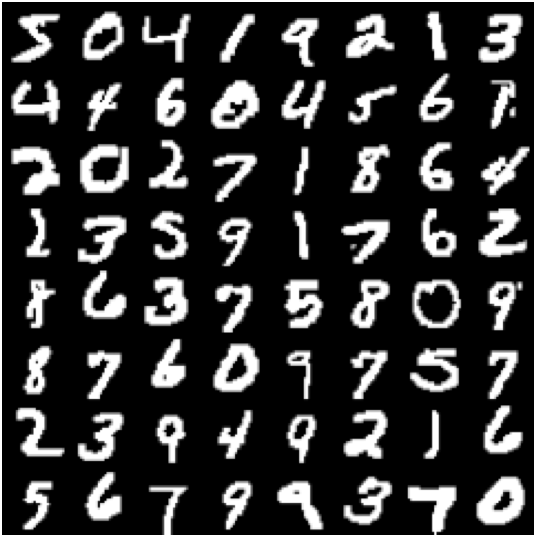
\includegraphics[width=0.5\textwidth]{mnist.png}
    \end{figure}
\end{frame}

\begin{frame}
    \frametitle{CIFAR-10}

    CIFAR-10 dataset consists 60,000 images in 10 classes \cite{krizhevsky2009}. There are 50,000 training images and 10,000 testing images.

    \begin{figure}
      \centering
      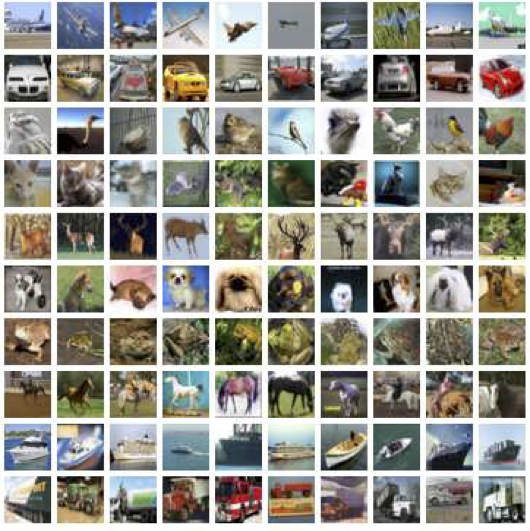
\includegraphics[width=0.5\textwidth]{cifar10.png}
    \end{figure}
\end{frame}

\begin{frame}
    \frametitle{Dataset: How to split the data?}

    \begin{itemize}
      \item[\ding{44}] If dataset has been splitted initially, please keep that way.
      \item[\ding{44}] If dataset comes as a whole, usually use 60\% as trianing data, 20\% as cross-validation and 20\% as testing data. 
      \item[\ding{44}] Another alternative is using 70\% as training data, 30\% as testing data.
    \end{itemize}
\end{frame}

\begin{frame}
    \frametitle{Dataset: Cross validation}

    \begin{itemize}
      \item[\ding{118}] Cross validation is used to keep track the performance of learning algorithm (overfitting? underfitting?).
      \item[\ding{118}] Used to be a small portion of training dataset, randomly selected.
      \item[\ding{118}] Serve as testing data when testing data is not visible.
      \item[\ding{118}] Help to choose and adjust parameters of the learning model.
    \end{itemize}
\end{frame}

\subsection{Data Standardization}

\begin{frame}
  \frametitle{Mean subtraction, Unit Variance}

  Let $\mu$ as mean image
  \begin{equation*}
    \mu=\frac{1}{m}\sum_{i=1}^{m} x^{(i)}
  \end{equation*}
  And then subtract mean image on every image:
  \begin{equation*}
    x^{(i)}=x^{(i)}-\mu
  \end{equation*}

  Let
  \begin{equation*}
    \sigma_{j}^{2}=\frac{1}{m}\sum_{i}\left(x_{j}^{(i)}\right)^{2}
  \end{equation*}
  and then
  \begin{equation*}
    x_{j}^{(i)}=\frac{x_{j}^{(i)}}{\sigma_{j}}
  \end{equation*}
  This is also called PCA whitening if it's applied to rotated data, the variance here can also be viewed as eigenvalues.
\end{frame}

\subsection{Principle Components Analysis}

\begin{frame}
    \frametitle{PCA}

    Principle Components Analysis (PCA) is a dimension reduction algorithm that can be used to significantly speed up unsupervised feature learning algorithm. PCA will find a lower-dimensional subspace onto which to project our data.

    Given a set of data $\bm{X}=\{x^{(1)}, x^{(2)}, \ldots, x^{(m)}\}$, where $x^{(i)}\in\mathbb{R}^{n}$, covariance is computed by
    \begin{equation*}
      \Sigma=\frac{\bm{X}\bm{X}^{\top}}{m}
    \end{equation*}

    Use eigendecomposition, we can obtain the eigenvectors $\bm{U}$:
    \begin{equation*}
      \bm{U}=\left[\begin{matrix}
          | & | & \cdots & | \\
          u_{1} & u_{2} & \cdots & u_{n} \\
          | & | & \cdots & |
        \end{matrix}\right]
    \end{equation*}
    and corresponding eigenvalues $\bm{\Lambda}=\{\lambda_{1}, \ldots, \lambda_{n}\}$. Note that usually $\bm{\Lambda}$ is a sorted in descending order.
\end{frame}

\begin{frame}
  \frametitle{PCA}

  Columns in $\bm{U}$ are principle bases, so that we can rotate our data to the new bases:
  \begin{equation*}
    \bm{X}_{\text{rot}}=\bm{U}^{T}\bm{X};
  \end{equation*}
  Noted that $\bm{X}=\bm{U}\bm{X}_{\text{rot}}$.

  To one of the data $x$, we can reduce the dimension by
  \begin{equation*}
    \tilde{x}=\left[\begin{matrix}
        x_{\text{rot}, 1} \\ \vdots \\ x_{\text{rot}, k} \\ 0 \\ \vdots \\ 0
      \end{matrix}\right]\approx \left[\begin{matrix}
        x_{\text{rot}, 1} \\ \vdots \\ x_{\text{rot}, k} \\ x_{\text{rot},k+1} \\ \vdots \\ x_{\text{rot}, n}
      \end{matrix}\right]=x_{\text{rot}}
  \end{equation*}
  
  The resulted $\tilde{\bm{X}}$ can approximate the distribution of $\bm{X}_{\text{rot}}$ since it's dropping only small components. And we reduced $n-k$ dimensions of the original data
\end{frame}

\begin{frame}
  \frametitle{PCA}

  We can recover the approximation of original signal $\hat{\bm{X}}$ from $\tilde{X}$:
  \begin{equation*}
    \hat{x}=U\left[\begin{matrix}
        \tilde{x}_{1} \\ \vdots \\ \tilde{x}_{k} \\ 0 \\ \vdots \\ 0
      \end{matrix}\right]
  \end{equation*}
\end{frame}

\begin{frame}
  \frametitle{PCA: Number of components to retain}

  To determine $k$, we usually look at the \emph{percentage of variance retained},

  \begin{equation}
    p=\frac{\sum_{i=1}^{k}\lambda_{j}}{\sum_{j=1}^{n}\lambda_{j}}
  \end{equation}

  One common heuristic is to choose $k$ so as to retain 99\% of the variance ($p\geq 0.99$).
\end{frame}

\subsection{ZCA Whitening}

\begin{frame}
    \frametitle{ZCA Whitening}

    ZCA whitening is just a recover version of PCA whitening:

    \begin{equation*}
      x_{\text{ZCA}}=Ux_{\text{PCA}}=U\frac{x_{\text{rot}}}{\sqrt{\bm{\Lambda}+\epsilon}}
    \end{equation*}
    where $\epsilon$ is a regularization term. When $x$ takes values around $[-1, 1]$, a value of $\epsilon\approx 10^{-5}$ might be typical.
\end{frame}

\section*{Q\&A}

\begin{frame}
  \frametitle{Q\&A}
  
  \begin{figure}
    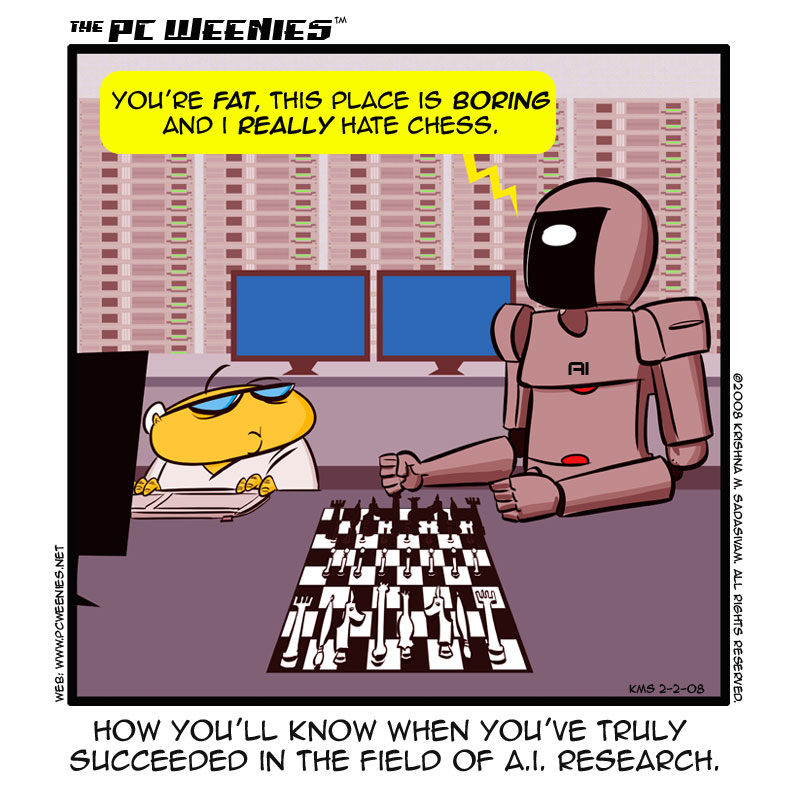
\includegraphics[width=0.6\textwidth]{ai_jokes.jpg}
  \end{figure}
\end{frame}

\begin{frame}
  \frametitle{References}
  \footnotesize
  \bibliographystyle{apacite}
  \bibliography{../dlworkshopref}
\end{frame}

\end{document}
%%% Local Variables:
%%% mode: latex
%%% TeX-master: t
%%% End:
